\documentclass[a4paper,12pt]{report}
\usepackage{mathptmx}
\usepackage[utf8]{inputenc}
\usepackage[hidelinks]{hyperref} % for citation
\hypersetup{
    colorlinks=true,
    linkcolor=blue,
    filecolor=magenta,      
    urlcolor=cyan,
    pdftitle={Overleaf Example},
    pdfpagemode=FullScreen,
    }
    
\setlength{\parskip}{1em}
\renewcommand{\baselinestretch}{1.25}

\setlength\parindent{0pt}
\usepackage{tikz}
\newcommand*\circled[1]{\tikz[baseline=(char.base)]{
            \node[shape=circle,draw,inner sep=2pt] (char) {#1};}}
            


\title{Report for the missions conducted during May to July at Nidelva in 2021}
\author{Yaolin Ge}
\date{July 2021}

\begin{document}

\maketitle

\subsection*{Manoeuvres}
\subsubsection*{Lawn-mower}
The AUV moves along the legs back and forth. The AUV is only exploring a certain depth, see Figure~\ref{fig:lawn_mower}. It is used for collecting data from a large area. 

Pros:
\begin{itemize}
    \item Large area can be explored.
    \item No potential loss of coverage. 
\end{itemize}

Cons:
\begin{itemize}
    \item Navigational issues, needs to pop-up during the mission if the duration of the entire lawn-mower mission is too long. 
    \item Time-consuming.
    \item Drift problem might lead to bad data aggregation.
    \item Depth variation is not captured.
\end{itemize}


\begin{figure}
    \centering
    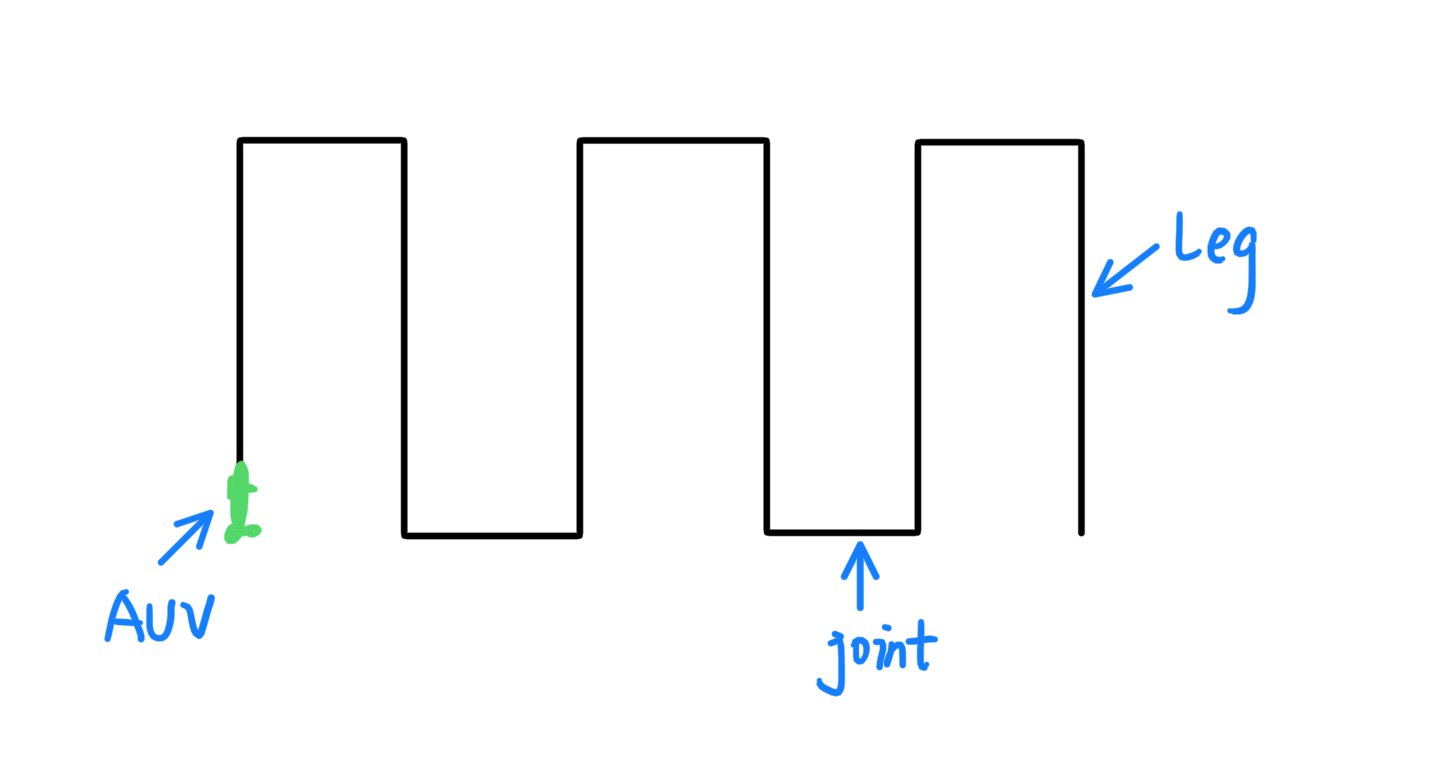
\includegraphics[width = \textwidth]{fig/lawn_mower.png}
    \caption{Lawn mower manoeuvre from the top view.}
    \label{fig:lawn_mower}
\end{figure}


\subsubsection*{Yo-Yo}
The AUV is moving up and down along the water column, see Figure~\ref{fig:yoyo}. It is used for collecting data in 3D water columns with relatively high efficiency. 

Pros:
\begin{itemize}
    \item Depth variation is captured. 
    \item Very efficient depth sampling.
    \item GPS calibration can be done every time when it is at the top point and the top point is close to the surface. 
\end{itemize}

Cons:
\begin{itemize}
    \item The constraints (pitch angle etc.) from the AUV determines that it cannot explore certain areas if they are in the dead zone (where Yo-Yo pattern does not pass).
    \item Data at each layers might be sparsely located, no local details. 
\end{itemize}


\begin{figure}
    \centering
    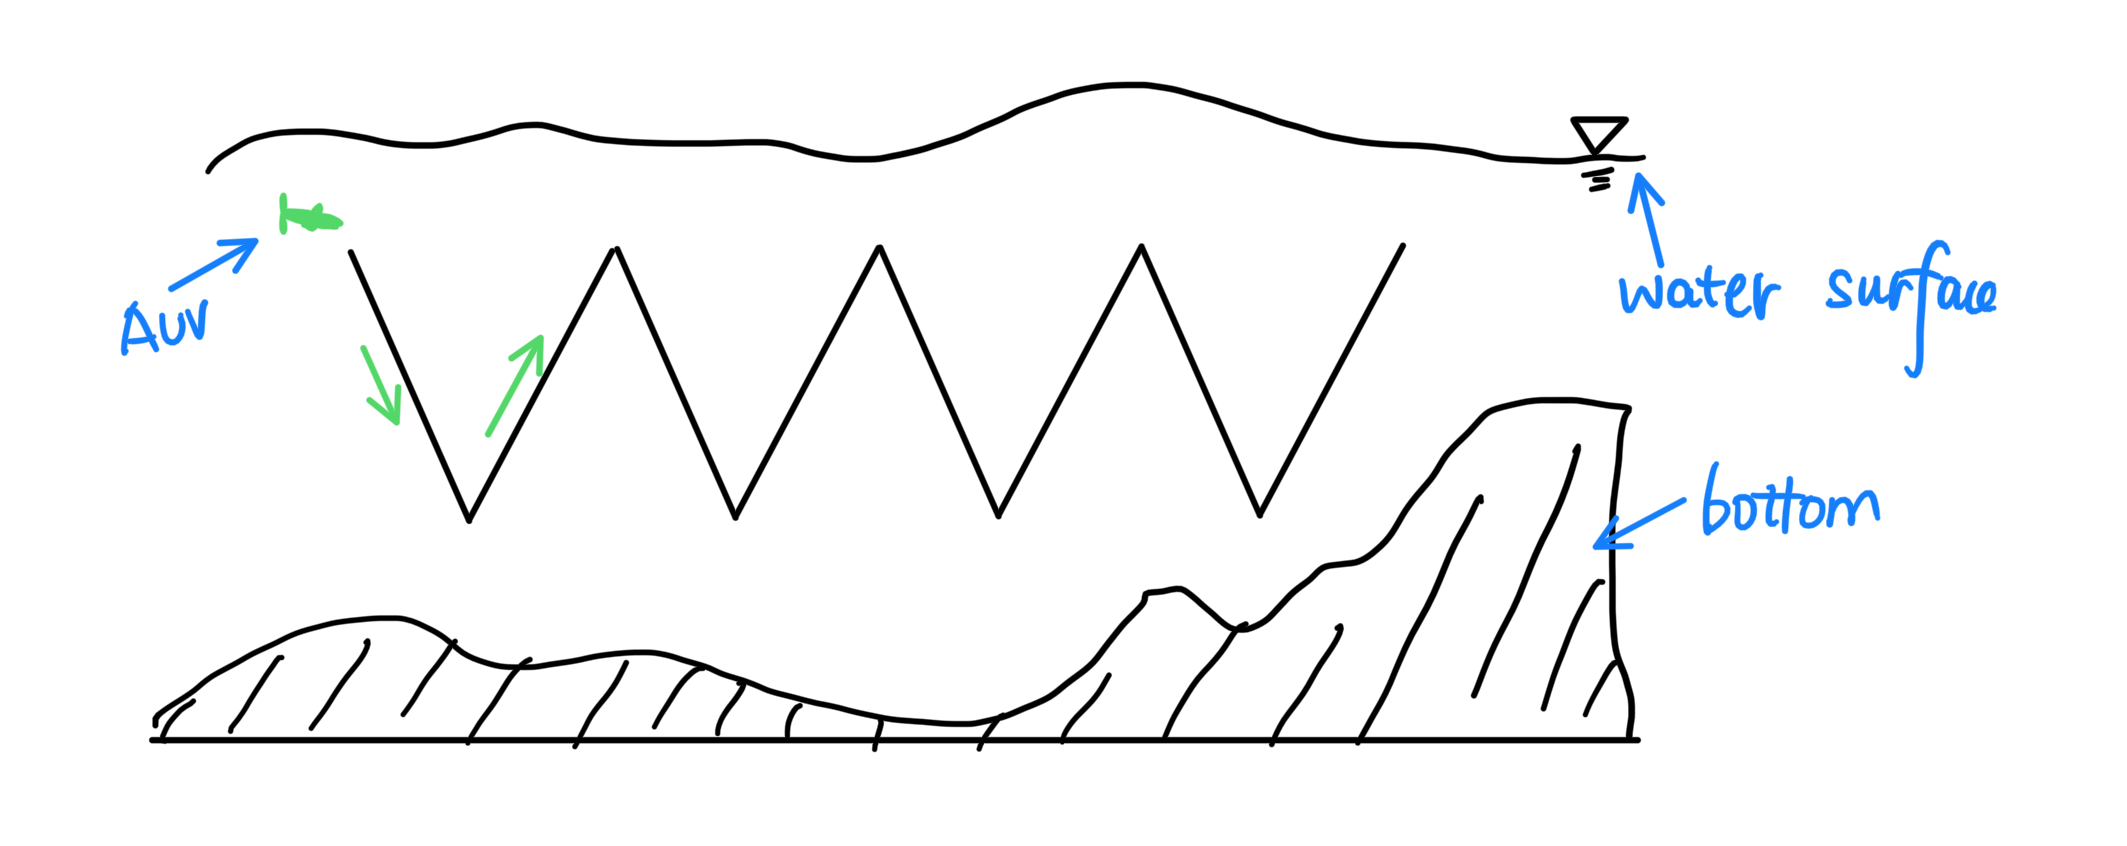
\includegraphics[width = \textwidth]{fig/yoyo.png}
    \caption{Yo-Yo manoeuvre from the side view.}
    \label{fig:yoyo}
\end{figure}

\subsubsection*{Elevator}

The AUV is taking a spiral elevator down to the bottom or up to the surface, see Figure~\ref{fig:elevator}. It is used for diving to the desired depth quickly. 

Pros:
\begin{itemize}
    \item Quickly dive to certain depth.
    \item Agile.
\end{itemize}
Cons:
\begin{itemize}
    \item The radius of the circle might be problematic when it is in some constrained areas.
    \item Sometimes hard to dive because of the lack of lifting force from the flap.
\end{itemize}

\begin{figure}
    \centering
    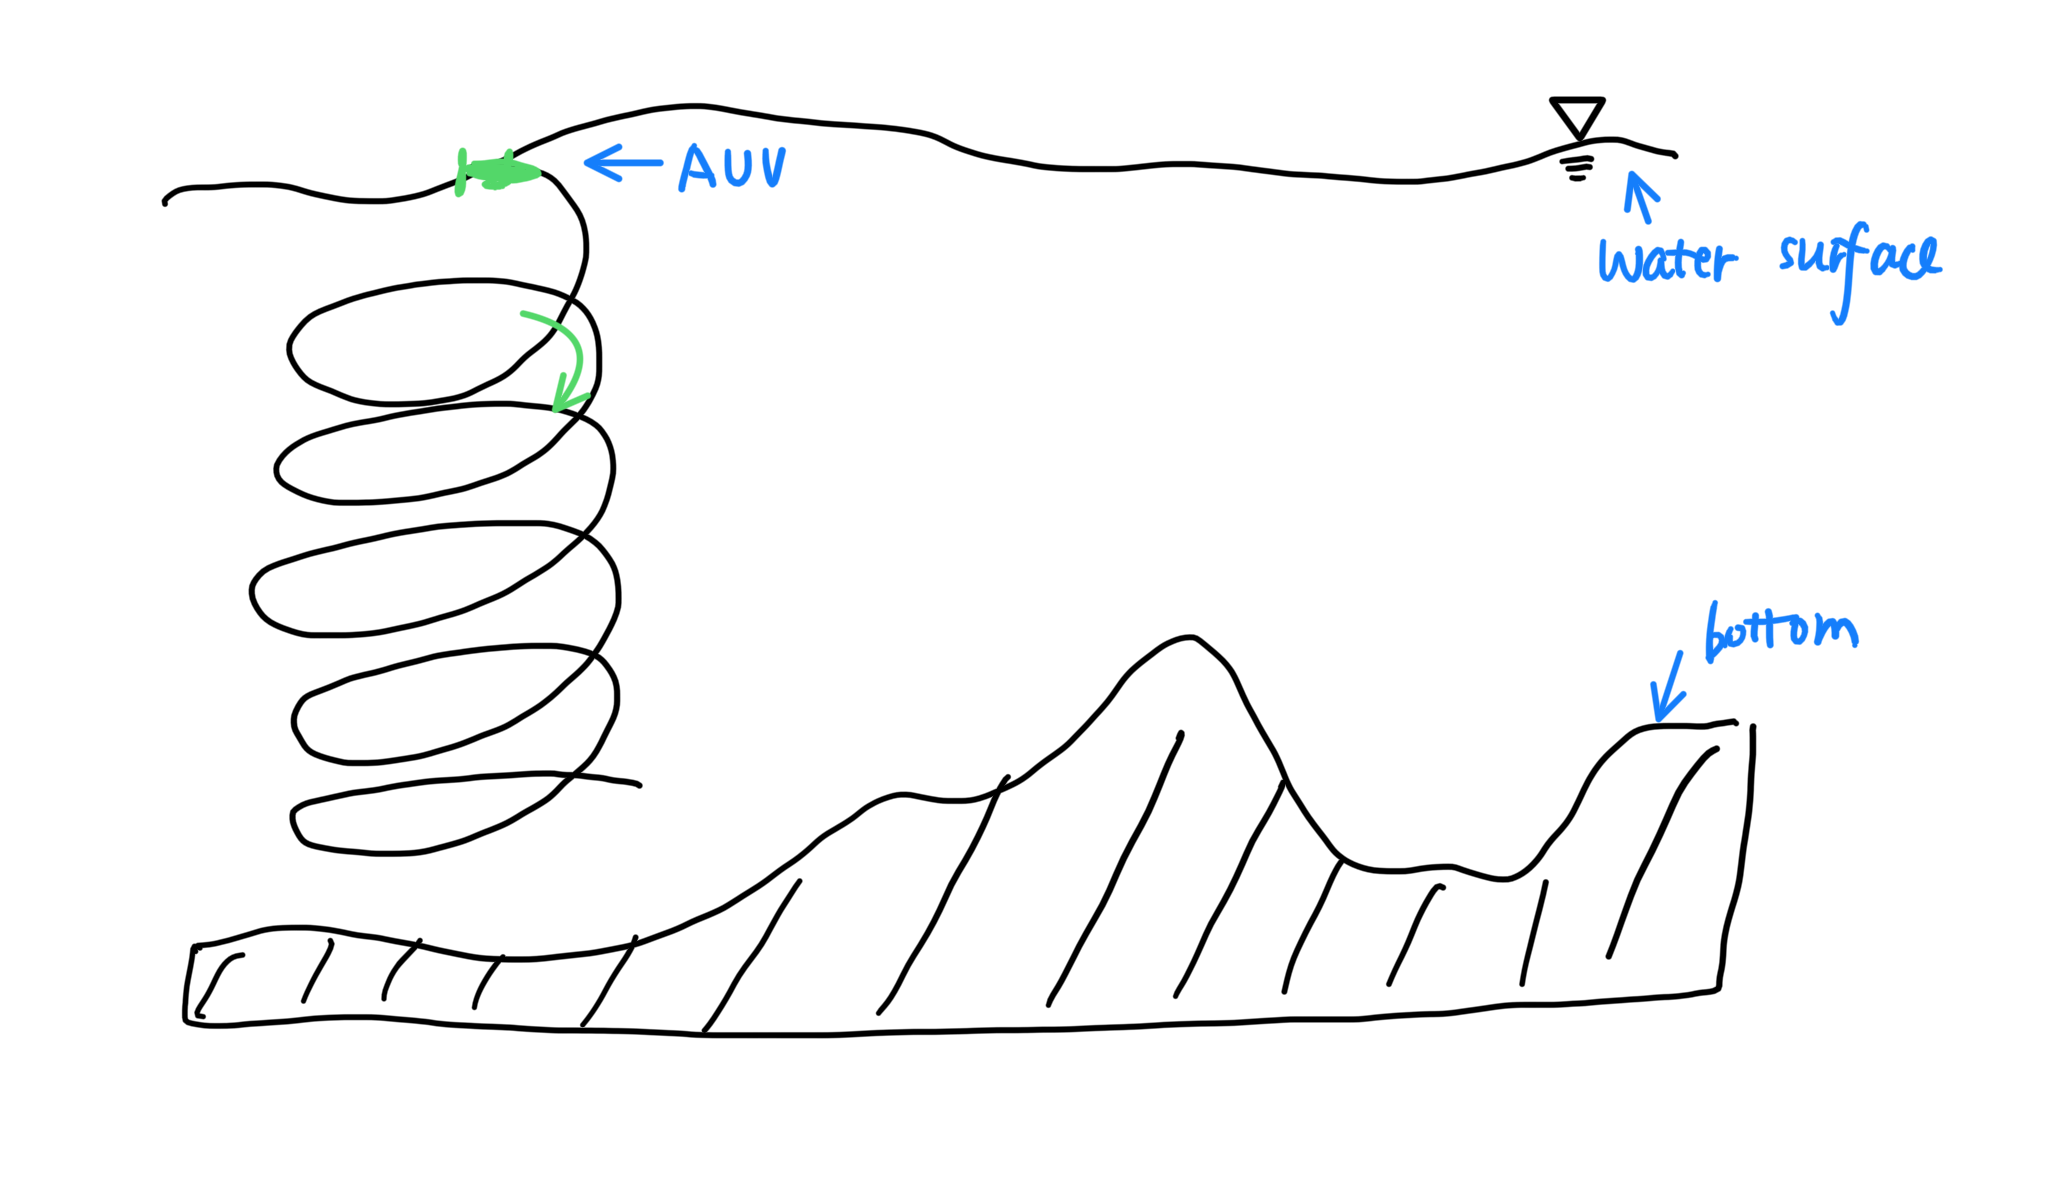
\includegraphics[width = \textwidth]{fig/elevator.png}
    \caption{Elevator manoeuvre from the side view.}
    \label{fig:elevator}
\end{figure}

\subsubsection*{Station-keeping}
The AUV is keeping its position at the surface by doing the loitering manoeuvre, see Figure~\ref{fig:station_keeping}. It is used for maintaining its position at the end of the mission or during the mission waiting for the next waypoint.


\begin{figure}
    \centering
    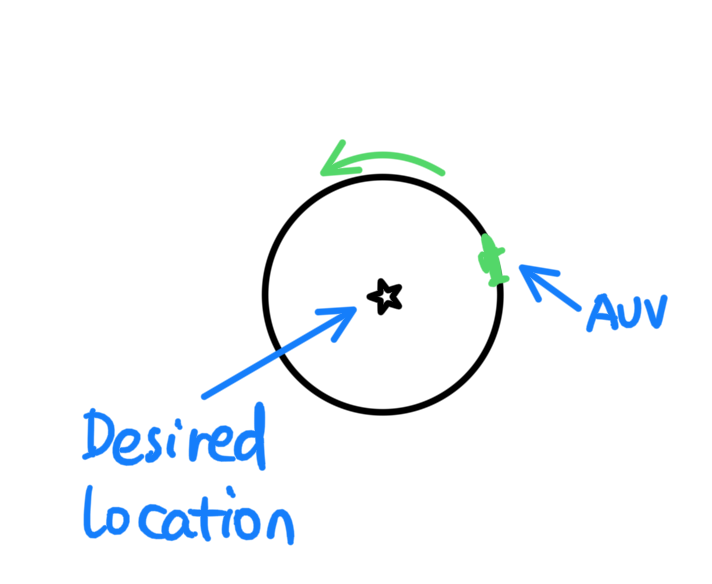
\includegraphics{fig/station_keeping.png}
    \caption{Station-keeping manoeuvre from the top view.}
    \label{fig:station_keeping}
\end{figure}


\subsubsection*{Pop-up}
The AUV pops up to the surface. It is used for GPS calibration. 

\end{document}